% Chapter Template

\chapter{Ensayos y resultados} % Main chapter title

\label{Chapter4} % Change X to a consecutive number; for referencing this chapter elsewhere, use \ref{ChapterX}

%----------------------------------------------------------------------------------------
%	SECTION 1
%----------------------------------------------------------------------------------------

Este capítulo se presentan los ensayos realizados para verificar la funcionalidad de los componentes individuales y del sistema completo, junto con el análisis de los resultados obtenidos.

\section{Banco de pruebas}

En esta sección se describe el entorno de pruebas que se creó para simular y evaluar el rendimiento del sistema en condiciones controladas. El objetivo del banco de pruebas fue verificar la correcta comunicación entre los nodos sensores, el módulo de relés y el gateway, asegurando que los datos fluyeran de manera precisa y que el sistema reaccionara adecuadamente a los comandos.

Para recrear este entorno, se utilizaron dos nodos sensores, el sensor LM35 y el el sensor MHZ19. Además, se integró un nodo con un módulo de relés, cuyos estados fueron simulados mediante leds, lo que facilitó la visualización de los cambios.

La transmisión de los datos desde los nodos hacia el gateway se realizó mediante el protocolo ESP-NOW, lo que permitió una comunicación inalámbrica eficiente entre los dispositivos. Los nodos sensores capturaron la información ambiental y la enviaron al gateway, mientras que el nodo de relés reportó el estado actual de los relés utilizando también ESP-NOW.

El gateway, estuvo conectado a una computadora para monitorear la recepción de los datos a través de la consola, validando que toda la información llegara correctamente. Este enfoque permitió realizar un seguimiento detallado del funcionamiento de los componentes y su interacción dentro del sistema.

En la figura \ref{fig:banco_pruebas} se puede visualizar los componentes utilizados para el banco de pruebas. 

\begin{figure}[H]
\centering 
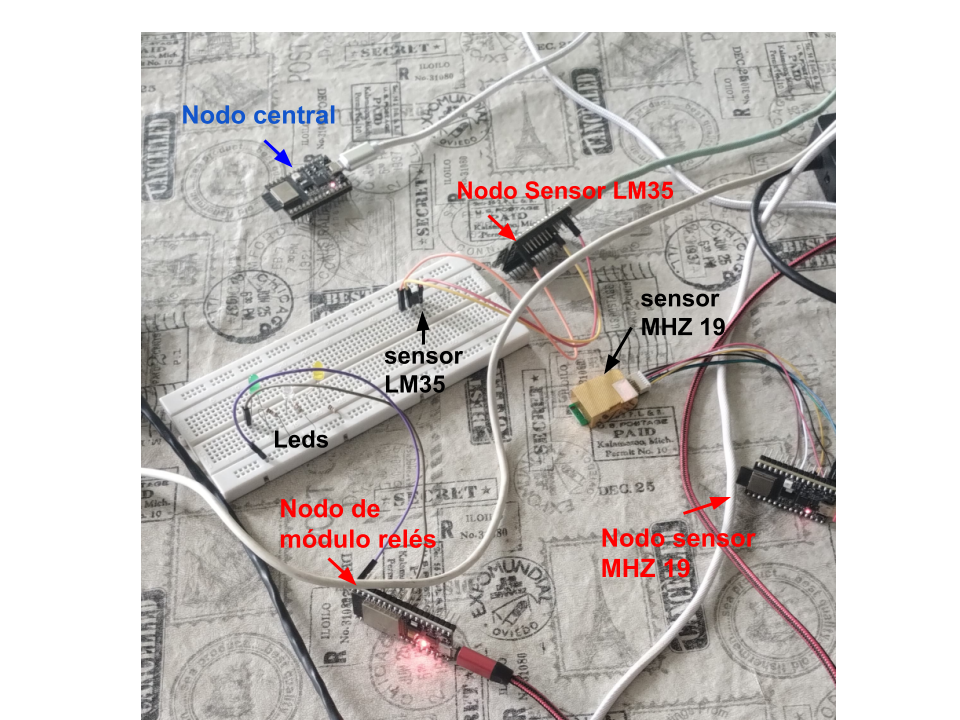
\includegraphics[width=0.9\textwidth]{./Figures/banco_pruebas.png}
\caption{Prototipo utilizado para las pruebas.}
\label{fig:banco_pruebas}
\end{figure}



%----------------------------------------------------------------------------------------

\section{Prueba de componentes}

Para asegurar el correcto funcionamiento de los sensores y del módulo de relés, se llevaron a cabo diversas pruebas de hardware y software. Estas pruebas fueron esenciales para validar que los sensores capturaran los datos correctamente y que el módulo de relés respondiera adecuadamente a los comandos recibidos, garantizando así una comunicación precisa entre estos componentes dentro del sistema.

\subsection{Prueba de sensores}

Se realizaron pruebas para verificar la precisión de los sensores LM35 y MHZ19 en la recolección de datos de temperatura y CO2. Los ensayos incluyeron:

\begin{itemize}
	\item Prueba de medición individual: se conectaron los sensores a un nodo de manera individual y se comprobó que los valores de temperatura y CO2 obtenidos fueran coherentes con las condiciones ambientales actuales. 
	\item Prueba de transmisión de datos: una vez que los sensores recolectaron los datos, se probó la transmisión de estos al gateway a través del protocolo ESP-NOW. Se monitoreó la consola del gateway para verificar que los datos llegaran sin pérdidas o alteraciones en el tiempo esperado.
\end{itemize}

\subsubsection{Resultados}

Para el sensor LM35, se aplicó un secador de pelo sobre el sensor para generar variaciones de temperatura. Los resultados de esta prueba se muestran en la figura \ref{fig:datos_lm35}, donde se puede observar claramente el cambio en los valores de temperatura registrados.

\begin{figure}[H]
\centering 
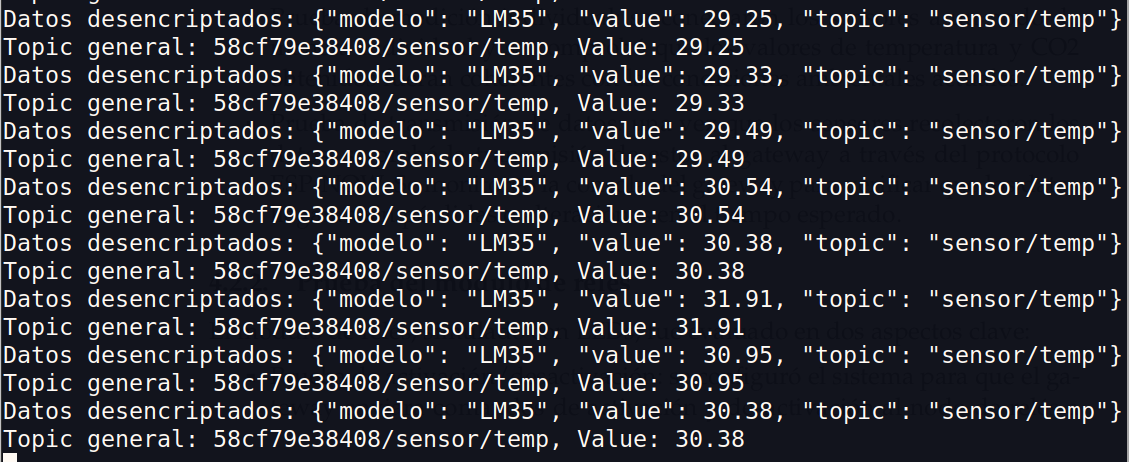
\includegraphics[width=0.8\textwidth]{./Figures/datos_lm35.png}
\caption{Datos del sensor LM35.}
\label{fig:datos_lm35}
\end{figure}

En el caso del sensor MHZ19, se generó una variación en la concentración de CO2 mediante una reacción química entre vinagre y bicarbonato de sodio, que liberó CO2. Los datos de esta variación se pueden ver en la figura \ref{fig:datos_mhz19}, con un comportamiento coherente ante el incremento de CO2.

\begin{figure}[H]
\centering 
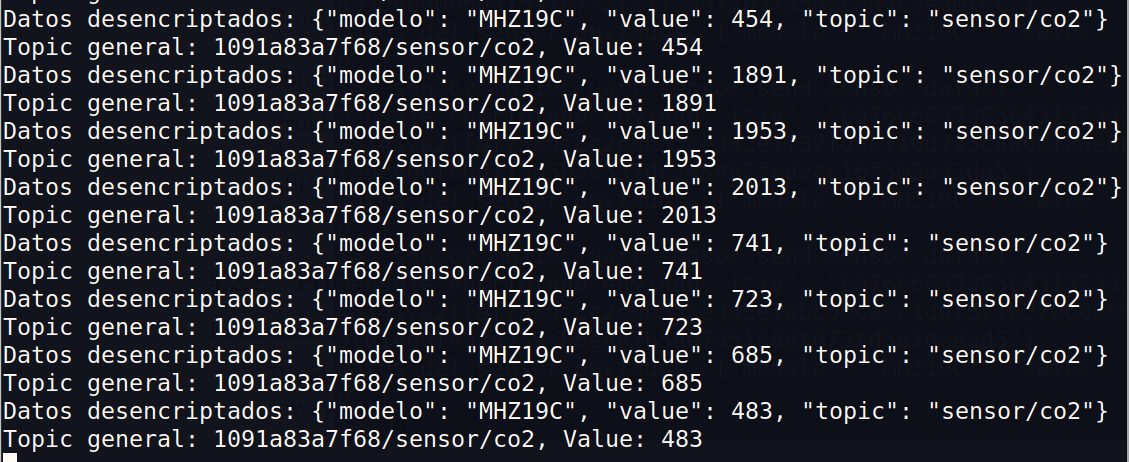
\includegraphics[width=0.8\textwidth]{./Figures/datos_mhz19.png}
\caption{Datos del sensor MHZ19.}
\label{fig:datos_mhz19}
\end{figure}

En ambas pruebas, los datos recolectados por los sensores fueron transmitidos exitosamente al gateway, sin pérdidas ni errores, confirmando la estabilidad y confiabilidad del sistema en la transmisión de la información.


\subsection{Prueba del módulo de relés}

El módulo de relés, simulado con LEDs, fue evaluado en dos aspectos clave:

\begin{itemize}
	\item Prueba de activación/desactivación: se configuró el sistema para que el gateway enviara comandos de activación y desactivación al nodo de relés a través de ESP-NOW. Se observó que los LEDs respondían correctamente a los comandos, encendiéndose y apagándose de manera precisa.
	\item Prueba de sincronización: para asegurar que los estados de los relés se mantuvieran sincronizados con el sistema, se verificó que los cambios en los LEDs correspondieran con los comandos enviados por el gateway sin retrasos significativos.
\end{itemize}

\subsubsection{Resultados}

En la figura \ref{fig:prueba_rele}, se muestra el proceso de envío de comandos desde el gateway hacia el nodo de relés. En primer lugar, el gateway envió un comando para activar el relé, lo que fue recibido correctamente por el nodo, encendiendo el led azul que simula el funcionamiento del relé. Posteriormente, se envió el comando de desactivación por lo que el nodo apagó el led correspondiente.

\begin{figure}[H]
\centering 
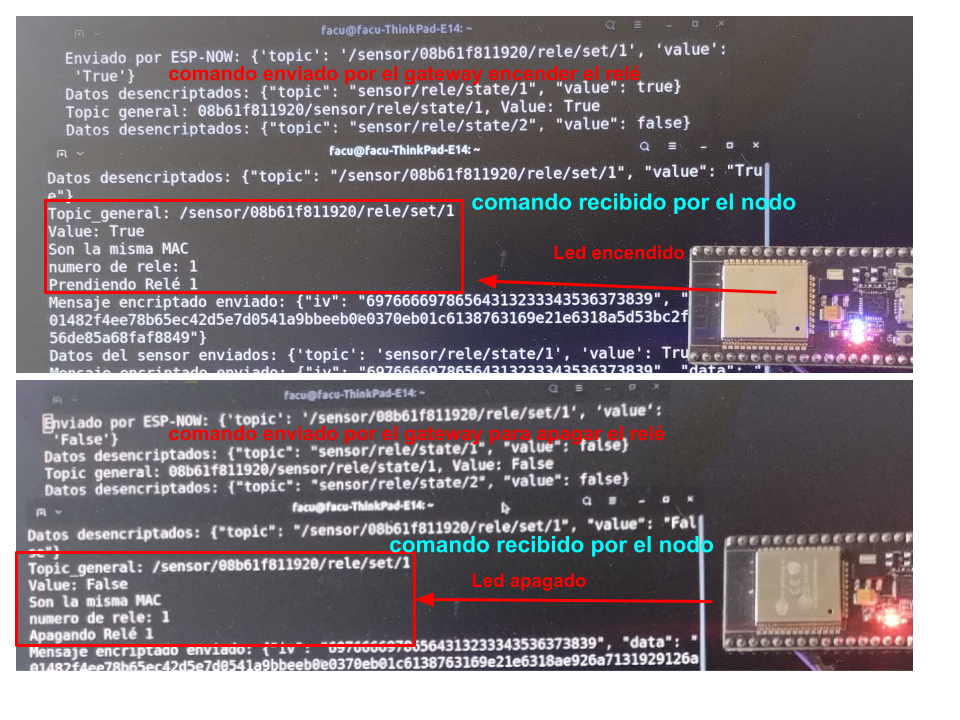
\includegraphics[width=1\textwidth]{./Figures/prueba_rele.png}
\caption{Prueba relé.}
\label{fig:prueba_rele}
\end{figure}

Los resultados de las pruebas de activación/desactivación y sincronización fueron satisfactorios. Los leds respondieron de forma precisa a los comandos enviados, encendiéndose y apagándose sin errores. Además, los cambios en el estado del relé se realizaron sin retrasos significativos.


%----------------------------------------------------------------------------------------

\section{Pruebas del sistema: Microcontrolador y Firmware}

En esta sección se describen las pruebas realizadas sobre el microcontrolador ESP32-C3 y su firmware, evaluando tanto la funcionalidad del hardware como el rendimiento del software embebido.


\begin{itemize}
    \item Prueba de conectividad y comunicación: se verificó que los nodos sensores y el nodo de relés, basados en ESP32-C3, pudieran establecer conexiones estables mediante ESP-NOW con el gateway. En la figura \ref{fig:con_sen_get}, se puede observar cómo el nodo sensor y el nodo del módulo de relés lograron establecer una conexión exitosa con el gateway.
    
\begin{figure}[H]
\centering 
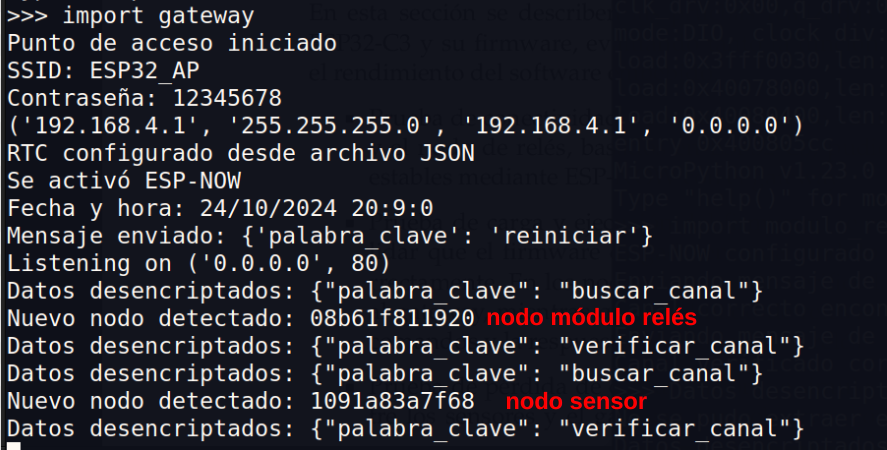
\includegraphics[width=0.8\textwidth]{./Figures/conexion_s_g.png}
\caption{Conexión de nodos al gateway.}
\label{fig:con_sen_get}
\end{figure}
    
    \item Prueba de carga y ejecución del firmware: se realizaron pruebas para validar que el firmware cargado en cada módulo ESP32-C3 se ejecutara correctamente. En los nodos sensores, se verificó la captura y envío de datos al gateway, mientras que en el nodo de relés se comprobó la recepción de comandos y la respuesta adecuada de los relés. Estos ensayos ya fueron detallados previamente en la sección \textbf{Prueba de componentes}
    
    \item Prueba de fallos en el firmware: se simularon reinicios inesperados o fallos en la carga del firmware en los nodos ESP32-C3. Se evaluó la capacidad del sistema para reiniciar correctamente y recuperar la funcionalidad sin perder la conexión o los datos.
    
    \item Prueba de gestión de cambios de canal: se realizó una prueba para verificar que los nodos pudieran sincronizarse correctamente con el gateway después de un reinicio y posible cambio de canal. Al iniciar, el gateway envía un comando de reinicio a los nodos para asegurarse de que todos los dispositivos se encuentren en el mismo canal de comunicación. En la figura \ref{fig:comando_restart}, se puede observar el envío del comando de reinicio por parte del gateway.
   	
    
\begin{figure}[H]
\centering 
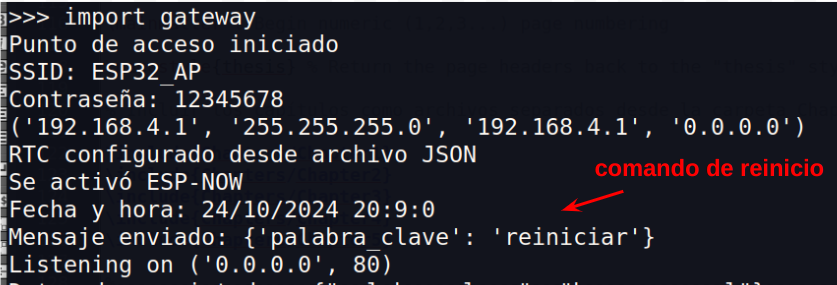
\includegraphics[width=0.8\textwidth]{./Figures/comando_restart.png}
\caption{Comando para reiniciar a los nodos.}
\label{fig:comando_restart}
\end{figure}

En la figura \ref{fig:nodo_restart}, se puede observar que el nodo de relés recibió el comando de reinicio enviado por el gateway de manera exitosa. Tras recibir el comando, el nodo se reinició y, al completar el proceso de arranque, encontró y se conectó al canal correcto, restableciendo la comunicación con el gateway sin inconvenientes.

\begin{figure}[H]
\centering 
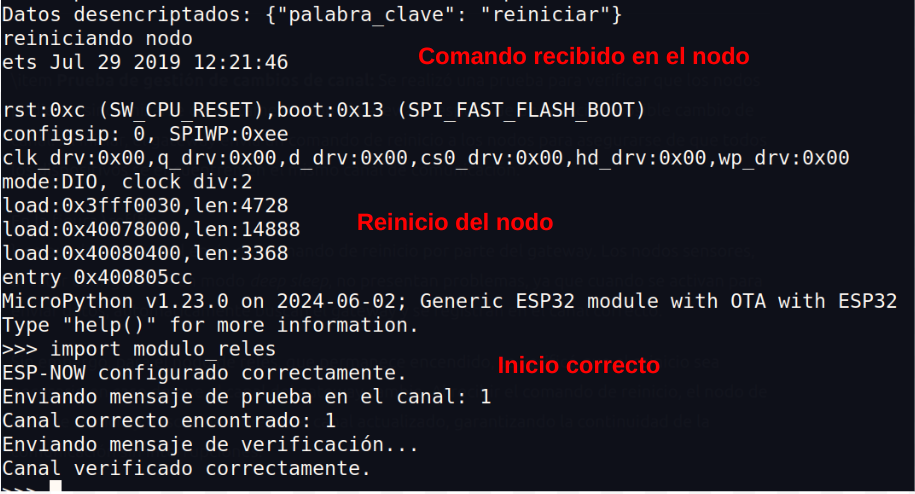
\includegraphics[width=0.8\textwidth]{./Figures/nodo_restart.png}
\caption{Nodo reiniciado.}
\label{fig:nodo_restart}
\end{figure}


    
    
\end{itemize}


%----------------------------------------------------------------------------------------


\section{Pruebas sobre la aplicación web progresiva}

En esta sección se describen las pruebas realizadas sobre la aplicación web progresiva (PWA) desarrollada para el monitoreo y gestión remota del sistema. Las pruebas incluyen la validación de las funcionalidades clave de la PWA, tales como la autenticación de usuarios, la visualización de datos de sensores, el control de los relés y la configuración de parámetros.

\subsection{Prueba de inicio de sesión}

Se llevaron a cabo pruebas para validar el proceso de inicio de sesión en la PWA, tanto con credenciales válidas como inválidas. Los ensayos incluyeron:

\begin{itemize}
    \item Verificación con credenciales válidas: se ingresaron datos de acceso correctos (nombre de usuario y contraseña) y se comprobó que la aplicación permitiera acceder al sistema sin inconvenientes, redirigiendo al usuario a la interfaz principal.
    
    \item Verificación con credenciales inválidas: se ingresaron combinaciones de nombres de usuario y contraseñas incorrectas para asegurar que la PWA rechazara el acceso de manera adecuada. Como se muestra en la figura \ref{fig:error_login}, al intentar acceder con credenciales erróneas, la PWA devolvió un mensaje de error claro que indicaba "Usuario o contraseña incorrectos", sin permitir el acceso al sistema.


\begin{figure}[H]
\centering 
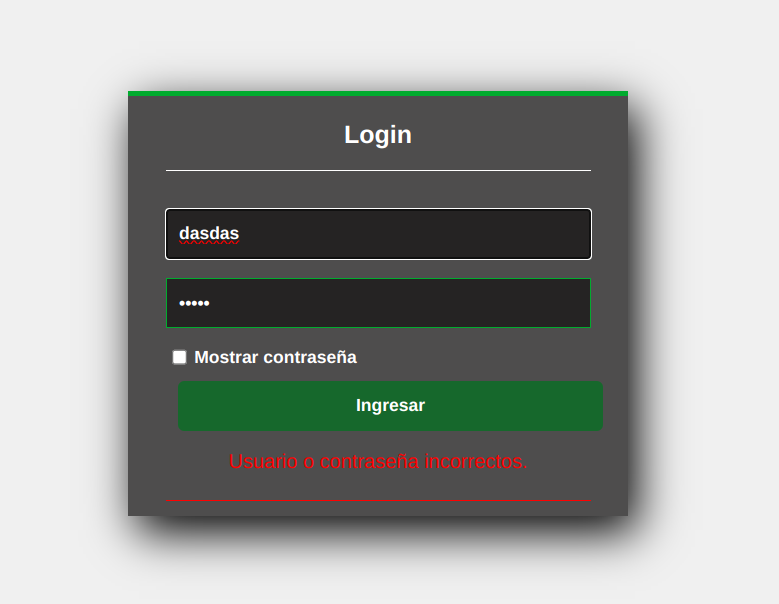
\includegraphics[width=0.7\textwidth]{./Figures/login_inc.png}
\caption{Error de login.}
\label{fig:error_login}
\end{figure}
   

\item Acceso sin iniciar sesión: Además, se probó la seguridad al intentar acceder a una URL o pantalla de la aplicación sin haber iniciado sesión previamente. Como se puede ver en la figura \ref{fig:ingreso_inv}, la PWA mostró un mensaje de alerta que indicaba "No tiene autorización para ingresar a esta pantalla", impidiendo el acceso a secciones no autorizadas del sistema.

\begin{figure}[H]
\centering 
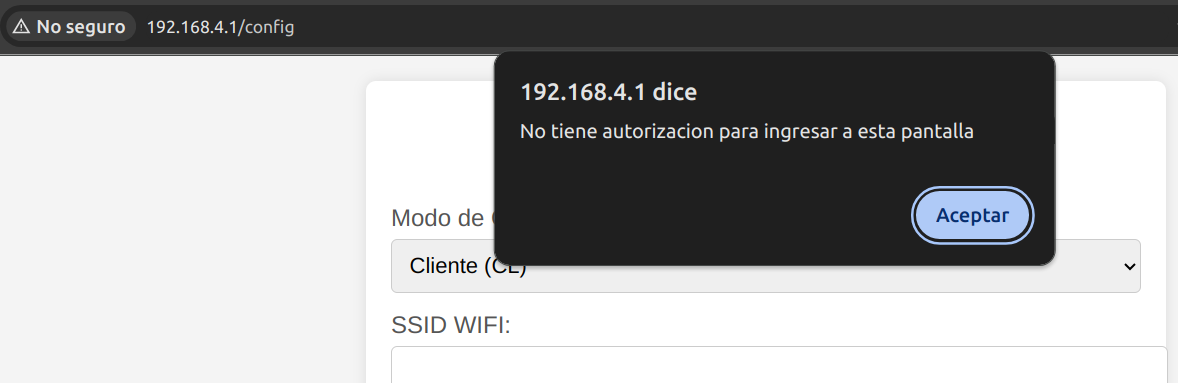
\includegraphics[width=0.9\textwidth]{./Figures/ingreso_inv.png}
\caption{Mensaje sin iniciar sesión.}
\label{fig:ingreso_inv}
\end{figure}

\end{itemize} 
   


\subsection{Prueba de visualización de datos de sensores}

Se realizaron pruebas para comprobar la precisión y actualización de los datos de los sensores que se muestran en la PWA. Las pruebas incluyeron:

\begin{itemize}
    \item Comparación con datos en consola: se visualizaron los datos de los sensores en la PWA y se compararon con los valores que se registraban simultáneamente en la consola del sistema. Se verificó que ambos datos coincidieran y se actualizaran en tiempo real sin inconsistencias. Esto se puede visualizar en la figura \ref{fig:datos_s_ok}.
    
\begin{figure}[H]
\centering 
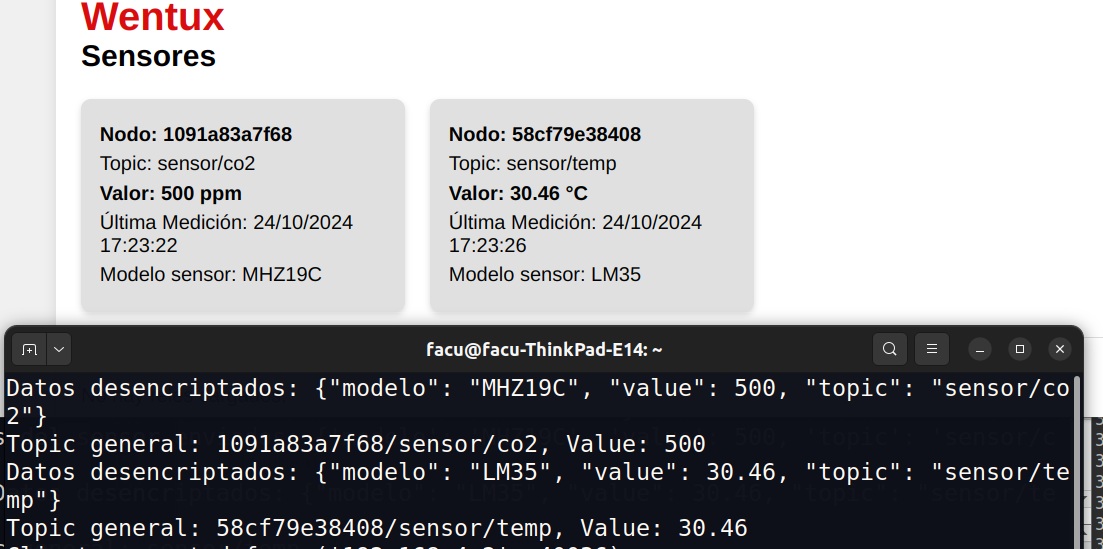
\includegraphics[width=0.9\textwidth]{./Figures/datos_sensores_ok.png}
\caption{Comparación de datos.}
\label{fig:datos_s_ok}
\end{figure}
    
    \item Verificación de actualización periódica: se comprobó que los datos de los sensores se actualizaran automáticamente en la interfaz de la PWA sin necesidad de recargar la página, asegurando que los valores reflejaran el estado más reciente de los sensores. En la figura \ref{fig:datos_p} se puede observar cómo los datos se reciben correctamente cada dos minutos, la diferencia de dos segundos entre mediciones se debe a un ligero retraso en el proceso de adquisición de datos por parte de los sensores.
    
    
\begin{figure}[H]
\centering 
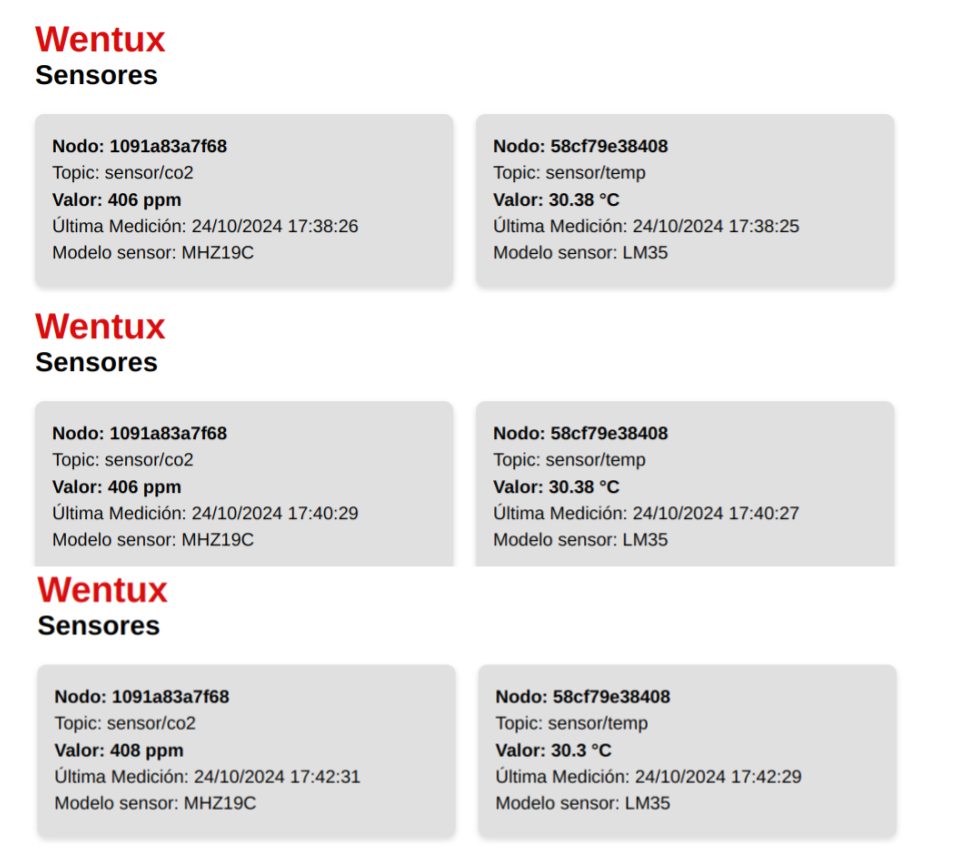
\includegraphics[width=0.8\textwidth]{./Figures/datos_periodicos.png}
\caption{Actualización periódica de datos.}
\label{fig:datos_p}
\end{figure}
    
\end{itemize}

\subsection{Prueba de control de relés}

El control de los relés desde la PWA fue evaluado para asegurar que los comandos enviados desde la interfaz se reflejaran correctamente en el hardware. Las pruebas incluyeron:

\begin{itemize}
    \item Sincronización con la consola: se compararon los estados de los relés mostrados en la PWA (on/off) con los registros de la consola del sistema, asegurando que ambos estuvieran sincronizados. Al activar o desactivar un relé desde la PWA, se verificó que los cambios también se reflejaran correctamente en la consola.
    
    \item Respuesta en tiempo real: se comprobó que los cambios en los estados de los relés se reflejaran casi instantáneamente en la PWA después de enviar el comando desde el gateway, asegurando que no hubiera retrasos significativos en la operación.
    
\end{itemize}

Como se muestra en la figura \ref{fig:pwa_rele}, los estados de los relés en la consola y en la PWA son idénticos, y los cambios se registran sin retrasos, lo que confirma el correcto funcionamiento del sistema.

\begin{figure}[H]
\centering 
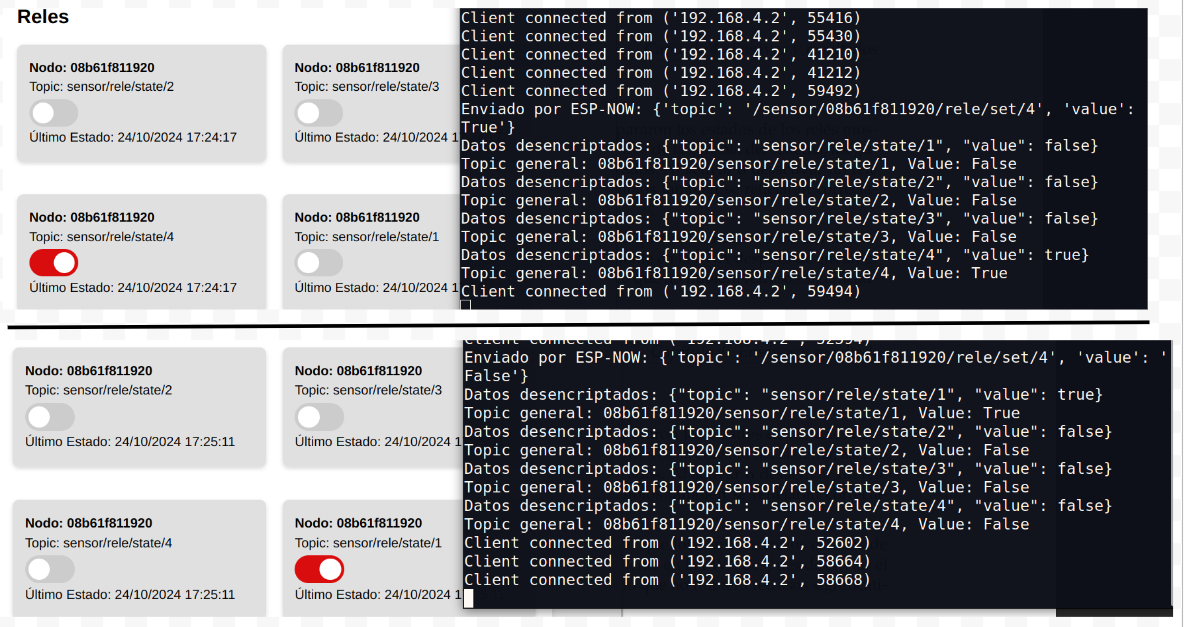
\includegraphics[width=1\textwidth]{./Figures/pwa_rele.png}
\caption{Prueba relés.}
\label{fig:pwa_rele}
\end{figure}

\subsection{Prueba de configuración}

La sección de configuración de la PWA fue evaluada para asegurar que los ajustes del sistema pudieran ser modificados correctamente y que los errores en la entrada de datos fueran gestionados de manera adecuada. La prueba realizada fue la siguiente:

\begin{itemize}
    \item Registro de errores en consola: se ingresaron datos incorrectos en los campos de configuración de la PWA para verificar que el sistema registrara estos errores de manera apropiada en la consola. Como se muestra en la figura \ref{fig:pwa_conf}, al introducir una contraseña de Wi-Fi incorrecta, el sistema registró un mensaje de error claro que indicaba 'contraseña incorrecta'. En respuesta a esto, el sistema cambió automáticamente al modo AP, permitiendo al usuario acceder nuevamente a la página de configuración para corregir el error y establecer los ajustes correctos.
\end{itemize}

\begin{figure}[H]
\centering 
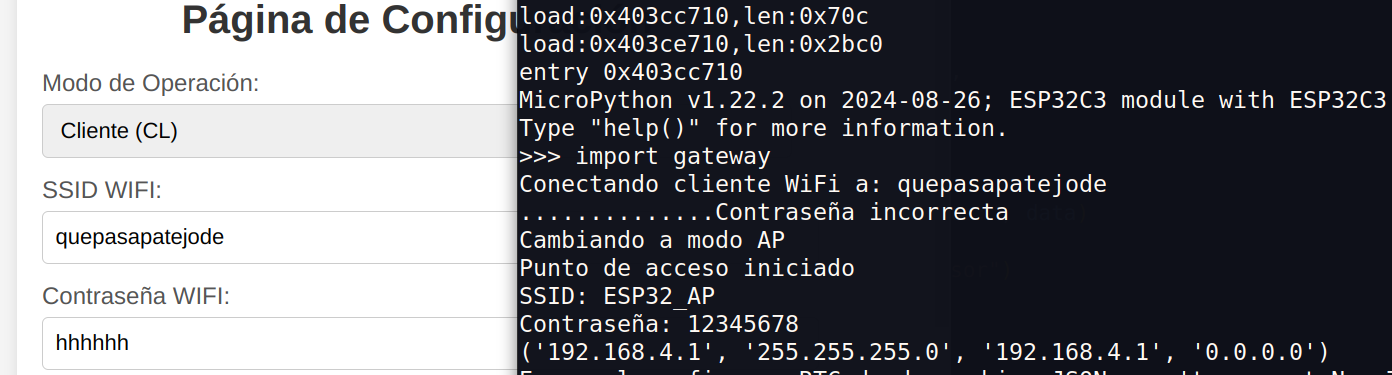
\includegraphics[width=1\textwidth]{./Figures/pwa_conf.png}
\caption{Registro de error.}
\label{fig:pwa_conf}
\end{figure}




%----------------------------------------------------------------------------------------

\section{Pruebas sobre el servidor OpenRemote}

Esta sección se describen las pruebas realizadas sobre el servidor IoT para verificar la recepción, almacenamiento y gestión de los datos provenientes de los sensores a través de un broker MQTT. Además, se valida el envío de comandos de control desde el servidor hacia el gateway para la operación de los relés.


\subsection{Pruebas de recepción de datos desde el broker MQTT}

\begin{itemize}
    \item Verificación de suscripción al \textit{broker} MQTT: se comprobó que el servidor OpenRemote estableciera una conexión exitosa con el \textit{broker} MQTT, paso fundamental para la recepción de datos de los sensores. En la figura \ref{fig:op_broker}, se puede observar tanto la consola del contenedor Docker, donde se registra la conexión correcta, como la interfaz web de OpenRemote, que confirma también el estado de conexión al \textit{broker}.
    
\begin{figure}[H]
\centering 
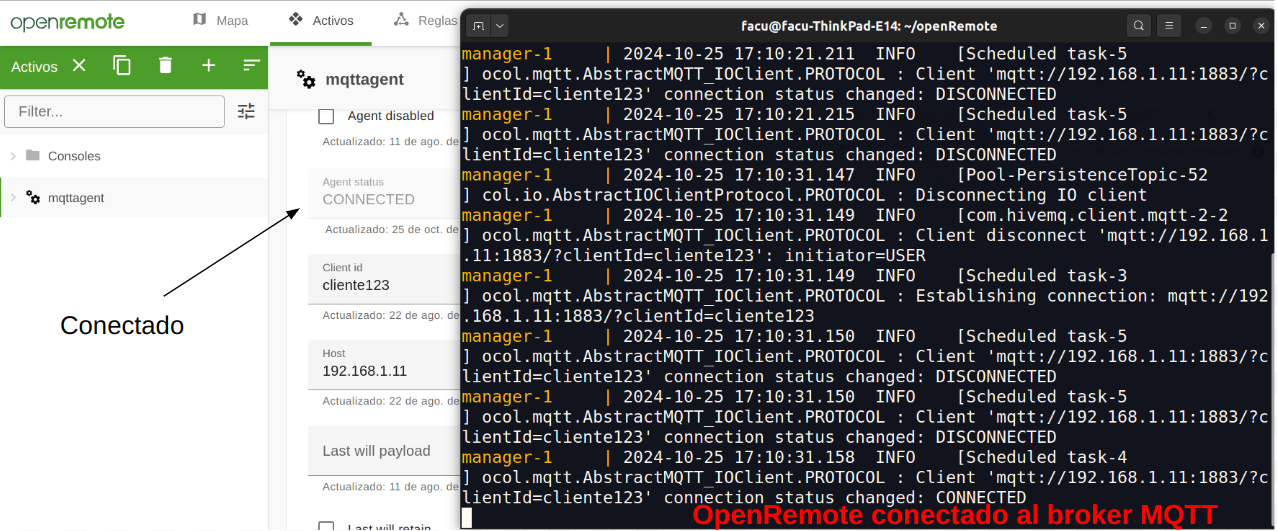
\includegraphics[width=1\textwidth]{./Figures/op_broker.png}
\caption{Verificación de conexión de openremote con el broker.}
\label{fig:op_broker}
\end{figure}

    
    \item Prueba de recepción de datos de sensores: se verificó que el servidor recibiera correctamente los datos de temperatura y CO2 enviados desde el gateway a través del \textit{broker} MQTT. En la figura \ref{fig:op_datos}, se muestra la interfaz de OpenRemote, donde los atributos de temperatura y CO2 están actualizados, y junto a ella, la interfaz de MQTT Explorer \citep{mqttexplorer}, confirmando que los valores recibidos por el \textit{broker} coinciden con los visualizados en OpenRemote. Esta coincidencia confirma que los datos se están transmitiendo y procesando correctamente desde el \textit{gateway} hasta el servidor.
    
    
\begin{figure}[H]
\centering 
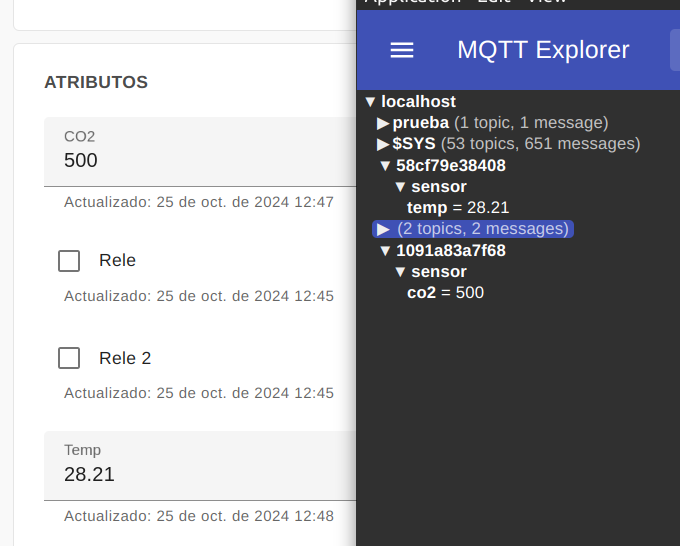
\includegraphics[width=0.7\textwidth]{./Figures/op_datos.png}
\caption{Recepción de datos en OpenRemote.}
\label{fig:op_datos}
\end{figure}   
    
    
    \item Prueba de actualización en tiempo real: se validó que los datos recibidos se actualizaran en tiempo real en el panel de control de OpenRemote, reflejando los cambios de los valores de los sensores sin necesidad de recargar la interfaz. Esto asegura que los usuarios puedan visualizar el valor más reciente de los sensores en el servidor.
    
\end{itemize}

\subsection{Pruebas de publicación de comandos a los relés}

\begin{itemize}
    \item Prueba de envío de comandos de control desde OpenRemote: se validó que el servidor pudiera enviar comandos al \textit{broker} MQTT para controlar los estados de los relés a través del \textit{gateway}. Al enviar un comando de activación/desactivación desde OpenRemote, se comprobó que el relé respondiera correctamente en tiempo real, sin retrasos significativos, y que el estado del relé se reflejara en la interfaz de OpenRemote. Esto se puede visualizar en la figura \ref{fig:op_reles}.
    
\begin{figure}[H]
\centering 
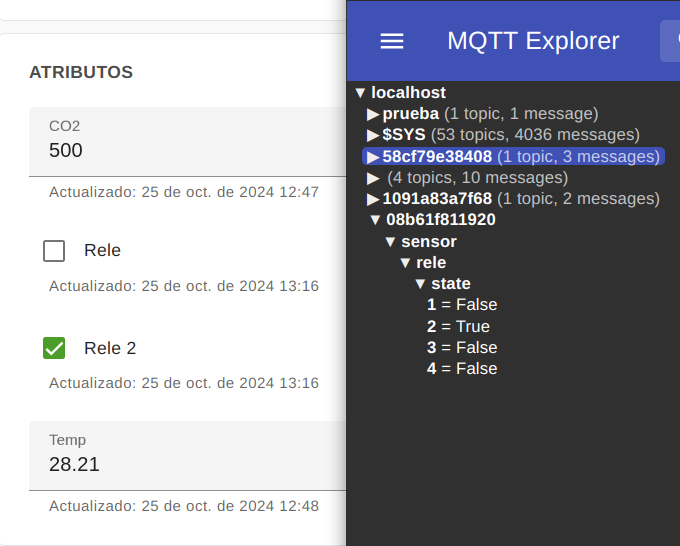
\includegraphics[width=0.6\textwidth]{./Figures/op_reles.png}
\caption{Envió de comandos desde OpenRemote.}
\label{fig:op_reles}
\end{figure}   
    
    \item Sincronización del estado de los relés en OpenRemote: se verificó que los cambios en el estado de los relés se actualizaran en la interfaz de OpenRemote, permitiendo a los usuarios verificar si los comandos fueron ejecutados correctamente en el hardware. Esto se observó mediante la comparación entre el estado mostrado en OpenRemote y el estado físico de los leds que simulan los relés. En la figura \ref{fig:op_rele}, se puede observar el cambio de estado del led que corresponde con lo que se visualiza en la interfaz de OpenRemote y Mqtt Explorer.
    
\begin{figure}[H]
\centering 
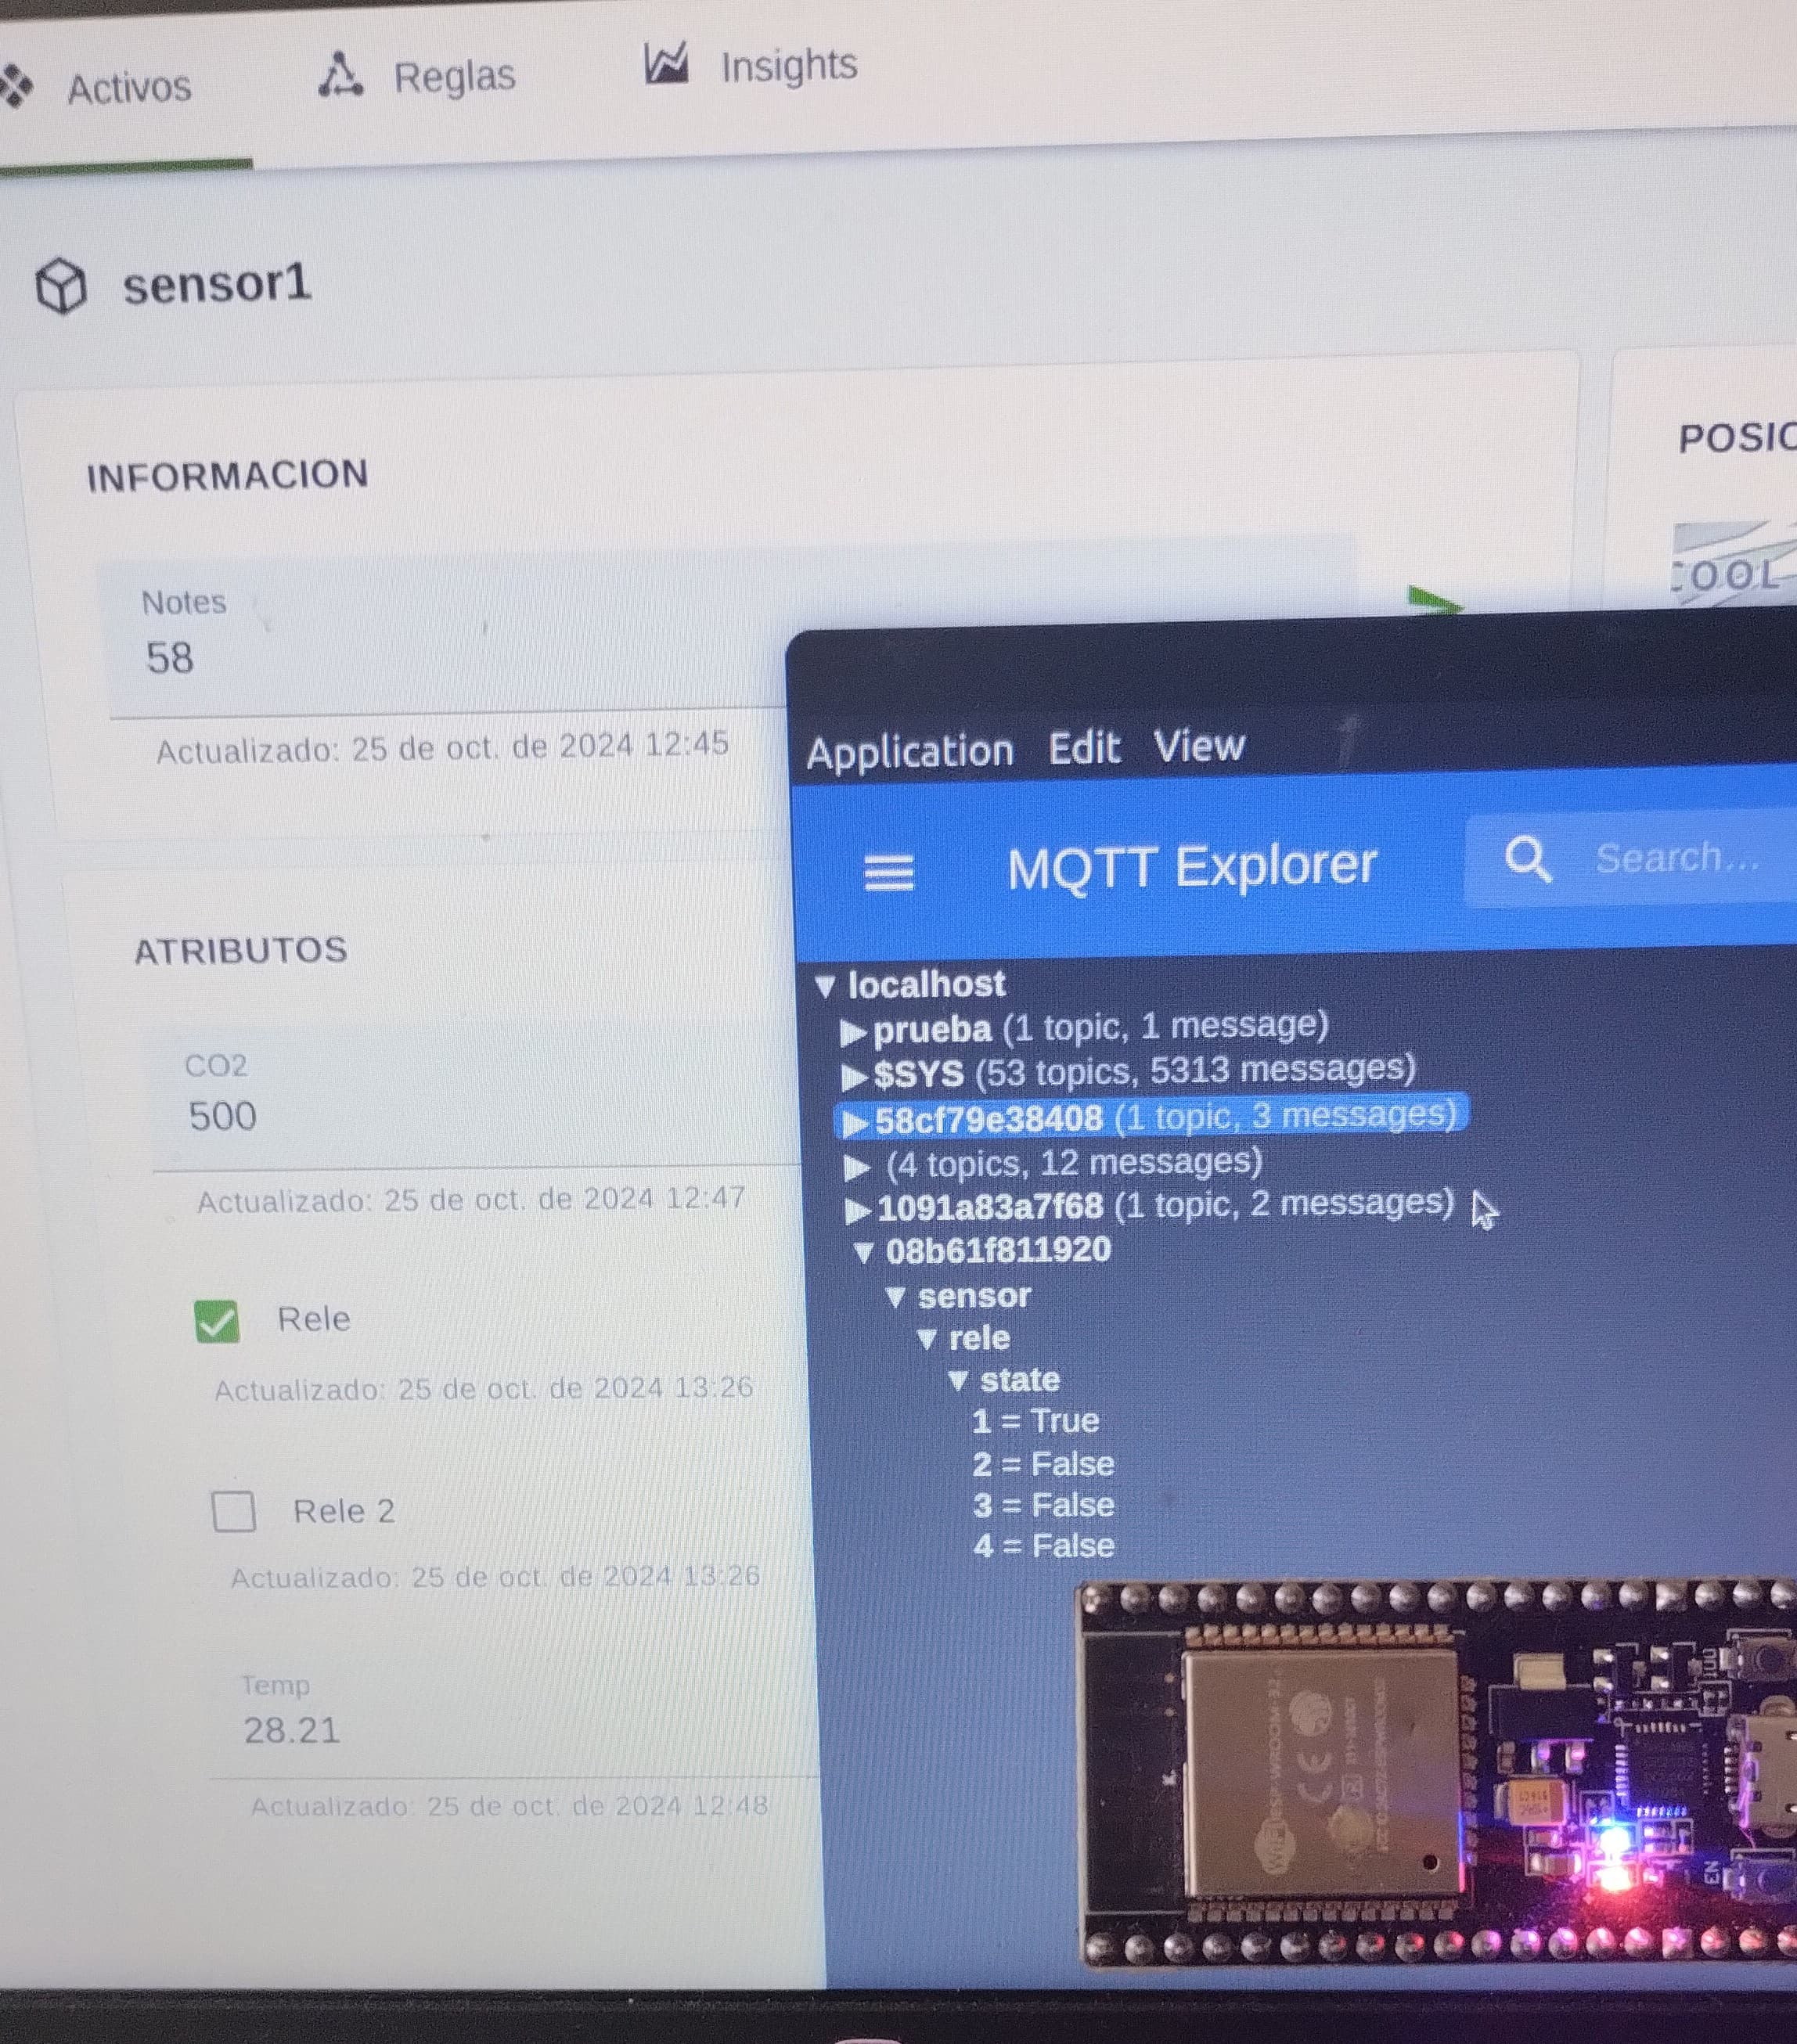
\includegraphics[width=0.6\textwidth]{./Figures/op_rele.png}
\caption{Verificación de cambio de estado del relé.}
\label{fig:op_rele}
\end{figure}  
    
    
\end{itemize}

\subsection{Pruebas de almacenamiento y gestión de datos}

\begin{itemize}
    \item Verificación de almacenamiento de datos: se comprobó que OpenRemote almacenara correctamente los datos recibidos en su base de datos interna, permitiendo su consulta en el historial y su análisis posterior. En la figura \ref{fig:op_historia}, se observa la interfaz de OpenRemote, que ofrece la opción de revisar el historial de datos. Esta funcionalidad permite seleccionar tanto el atributo específico como el periodo de tiempo que se desea analizar, facilitando el acceso a información detallada para el seguimiento y evaluación de los datos recopilados.

\begin{figure}[H]
\centering 
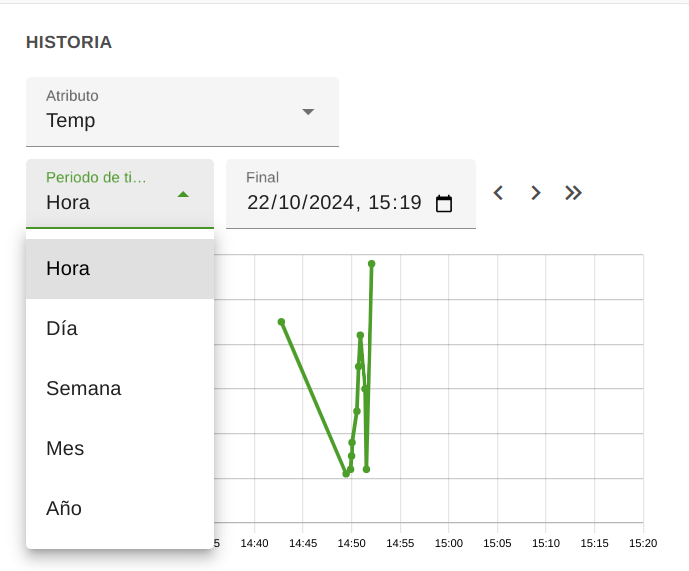
\includegraphics[width=0.6\textwidth]{./Figures/op_historia.png}
\caption{Opción de historia del atributo.}
\label{fig:op_historia}
\end{figure}  
    
    \item Prueba de visualización de datos históricos: se verificó que el sistema permitiera al usuario visualizar los datos históricos de los sensores, facilitando el monitoreo y análisis de las condiciones ambientales en un periodo extendido. En la figura \ref{fig:op_historial} se muestra un ejemplo de los datos históricos almacenados, evidenciando que el sistema puede gestionar grandes volúmenes de información sin comprometer el rendimiento.
    
\begin{figure}[H]
\centering 
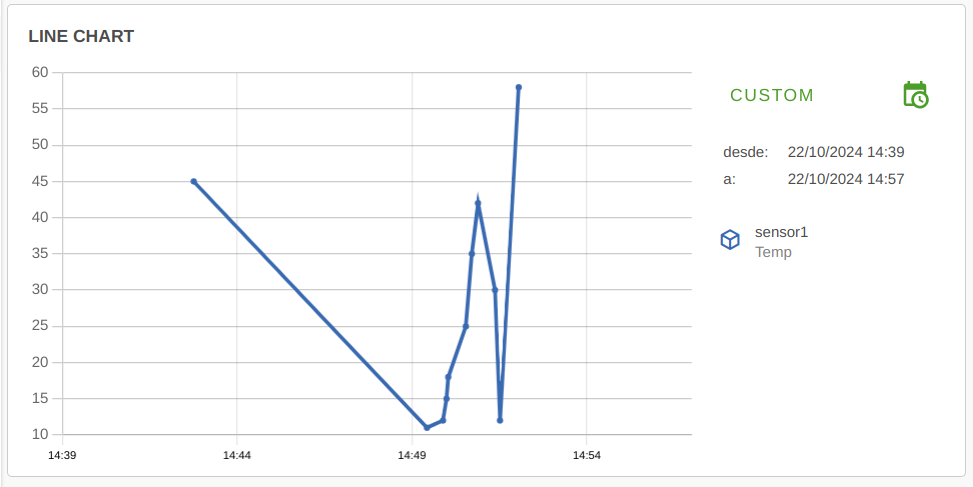
\includegraphics[width=0.9\textwidth]{./Figures/op_historial.png}
\caption{Grafico del sensor de temperatura.}
\label{fig:op_historial}
\end{figure}  
    
    
\end{itemize}




